\section{Offline$\leftrightarrow$Closed-Loop Correspondence (RQ2, part 2)}
\label{sec:linkage}

This section answers the second half of RQ2 -- does the offline candidate
ranking from Section~\ref{sec:characterization} correspond to the
closed-loop behavior in Section~\ref{sec:closed-loop}? -- and, jointly
with the horizon comparison below, RQ3's horizon question. Source:
\texttt{analysis/closed\_loop\_offline\_linkage\_20260914/}, computed with
two independent code paths in numerical agreement. \textbf{SIEVE has no
offline counterpart} (Section~\ref{sec:label-generation} defines labels
only for the continuation-policy family LRU/MRU/random) and is therefore
excluded from every comparison in this section; only MRU-vs-LRU and
random-vs-LRU are compared.

\textbf{RQ-CL1 (rank agreement).} At $H=16$, across the 10 family$\times$capacity
cells: MRU-vs-LRU agrees in sign (offline regret-gap sign matches
closed-loop miss-ratio-gap sign) in 7 of 10 cells, disagrees in 1, and is
tied on both sides (wiki2018) in 2; random-vs-LRU agrees in 6, disagrees
in 2, ties in 2. The discordant cells are always the same two:
\textbf{alibaba-block/cap32} (discordant for both pairs -- offline regret
gaps there are $-0.0027$ and $-0.0007$, i.e.\ barely non-zero on the
offline side too) and \textbf{metakv/cap128} (discordant for random-vs-LRU
only -- offline says random is very slightly worse than LRU, $+0.0013$
regret gap, while closed-loop shows random modestly beating LRU, $-0.015$
miss-ratio gap; Section~\ref{sec:closed-loop} additionally notes SIEVE
also beats LRU there). Excluding wiki2018's two trivially-tied cells,
concordance among the 8 non-degenerate cells is not manufactured by
wiki2018's automatic agreement: dropping wiki2018 still leaves the same
two discordant cells and the same qualitative picture.

\textbf{RQ-CL2 (gap-magnitude correspondence).} At $H=16$: MRU-vs-LRU
Pearson $r=0.835$ (Spearman $\rho=0.915$, Kendall $\tau=0.773$);
random-vs-LRU $r=0.755$ ($\rho=0.829$, $\tau=0.591$). Figure~\ref{fig:linkage-scatter}
shows both relationships directly, with the two discordant cells
annotated rather than hidden. These correlations rest on only 8--10
independent (family, capacity) points and are reported with that $n$
attached everywhere; they are not treated as population-scale estimates.

\begin{figure}[t]
  \centering
  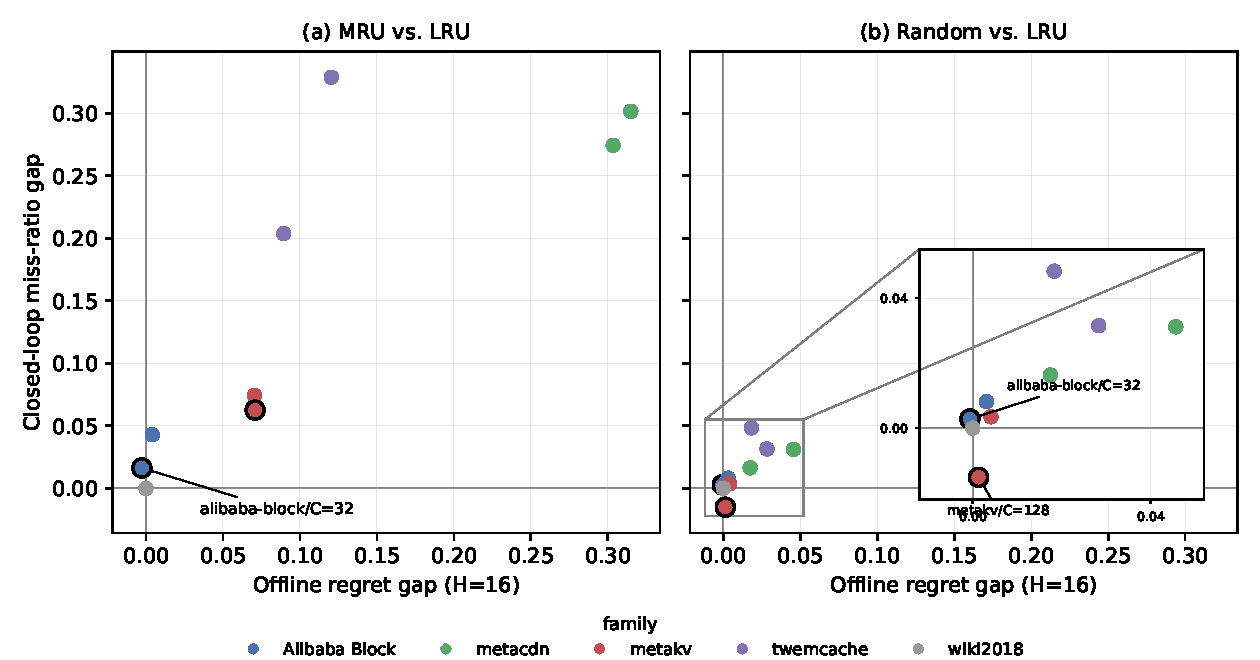
\includegraphics[width=\columnwidth]{figures/figure3_linkage_scatter.pdf}
  \caption{Offline regret gap vs.\ closed-loop miss-ratio gap, H=16, MRU-vs-LRU
  and random-vs-LRU. Reproducible from
  \texttt{paper/performance\_evaluation/scripts/figures/make\_figure3\_linkage\_scatter.py}
  against \texttt{outputs/rq\_cl2\_scatter\_data.csv}.}
  \label{fig:linkage-scatter}
\end{figure}

\textbf{RQ-CL3 (workload/capacity dependence).} metacdn and twemcache are
the strong-agreement, most-discriminative-offline regimes and also show
the largest closed-loop policy separation; alibaba-block is a
weak/ambiguous regime where the offline gap is close enough to zero that
its sign is not robust; metakv/cap128 is the one reversal regime; wiki2018
is degenerate on both sides, exactly, confirming it as a clean negative
control. An exploratory (not pre-registered) correlation between offline
discriminativeness ($1-\text{all-tied fraction}$) and closed-loop
$|\text{MRU}-\text{LRU}|$ separation, across all 10 cells at $H=16$, gives
Pearson $r=0.968$ -- Section~\ref{sec:mechanisms} traces this to a shared
underlying trace-locality property rather than treating it as a
coincidence.

\textbf{RQ-CL4 (horizon).} $H=16$ wins or ties on every magnitude-sensitive
statistic across every sensitivity slice tested (primary, excluding
wiki2018, test-window-only), for both pairs. The coarse concordant/
discordant/tied counts are \emph{identical} at $H=4$, $H=8$, and $H=16$
(the same two cells are discordant regardless of horizon); horizon changes
the \emph{strength} of the correspondence (the correlation coefficients
above), not which cells agree in sign. The differences between horizons
are modest in absolute terms ($r=0.746$ at $H=4$ to $r=0.835$ at $H=16$
for MRU-vs-LRU) and $n=8$--10 per horizon is small, but the pattern is
consistent and not cherry-picked.

\textbf{Answer to RQ2/RQ3.} Offline and closed-loop policy orderings agree
in the large majority of workload/capacity regimes where the offline
signal itself is not near zero, with two specific, characterized
exceptions; $H=16$ gives the strongest, though modest, alignment among the
three horizons tested. This is a bounded, evidenced claim, not a universal
predictive-validity claim for the offline labels.
